%%%%%%%%%%%%%%%%%%%%%%%%%%%%%%%%%%%%%%%%%
% Beamer Presentation
% LaTeX Template
% Version 2.0 (March 8, 2022)
%
% This template originates from:
% https://www.LaTeXTemplates.com
%
% Author:
% Vel (vel@latextemplates.com)
%
% License:
% CC BY-NC-SA 4.0 (https://creativecommons.org/licenses/by-nc-sa/4.0/)
%
%%%%%%%%%%%%%%%%%%%%%%%%%%%%%%%%%%%%%%%%%

%----------------------------------------------------------------------------------------
%	PACKAGES AND OTHER DOCUMENT CONFIGURATIONS
%----------------------------------------------------------------------------------------


\documentclass[
	11pt, % Set the default font size, options include: 8pt, 9pt, 10pt, 11pt, 12pt, 14pt, 17pt, 20pt
	%t, % Uncomment to vertically align all slide content to the top of the slide, rather than the default centered
	%aspectratio=169, % Uncomment to set the aspect ratio to a 16:9 ratio which matches the aspect ratio of 1080p and 4K screens and projectors
]{beamer}

\graphicspath{{Images/}{./}} % Specifies where to look for included images (trailing slash required)
\definecolor{codegreen}{rgb}{0,0.6,0}
\definecolor{codegray}{rgb}{0.5,0.5,0.5}
\definecolor{codepurple}{rgb}{0.58,0,0.82}
\definecolor{backcolour}{rgb}{0.95,0.95,0.92}
\usepackage{listings}
\usepackage{xcolor}
\lstdefinestyle{mystyle}{
    backgroundcolor=\color{backcolour},   
    commentstyle=\color{codegreen},
    keywordstyle=\color{magenta},
    numberstyle=\tiny\color{codegray},
    stringstyle=\color{codepurple},
    basicstyle=\ttfamily\footnotesize,
    breakatwhitespace=false,         
    breaklines=true,                 
    captionpos=b,                    
    keepspaces=true,                 
    numbers=left,                    
    numbersep=5pt,                  
    showspaces=false,                
    showstringspaces=false,
    showtabs=false,                  
    tabsize=2
}

\lstset{style=mystyle}

\usepackage{booktabs} % Allows the use of \toprule, \midrule and \bottomrule for better rules in tables
\usepackage{pgf}
\usepackage{tikz}
\usepackage{llvm/lang}  % include custom language for LLVM IR.
\usepackage{llvm/style}  % include custom style for Nasm
\usetikzlibrary{arrows,shapes,positioning,shadows,trees}
\tikzset{
  basic/.style  = {draw, text width=0.18\textwidth, drop shadow, font=\sffamily, rectangle},
  root/.style   = {basic, rounded corners=2pt, align=center,
                   fill=blue!30},
  level 2/.style = {basic, rounded corners=6pt, thin,align=center, fill=blue!40!green!20},
  level 3/.style = {basic, thin, align=left, fill=blue!10, text width=12.5em}
}

% Define block styles
\tikzstyle{decision} = [diamond, draw, fill=blue!20, 
    text width=4.5em, text badly centered, node distance=3cm, inner sep=0pt]
\tikzstyle{block} = [rectangle, draw, fill=blue!20, 
    text width=3.5em, text centered, rounded corners, minimum height=4em]
\tikzstyle{line} = [draw, -latex']
\tikzstyle{cloud} = [draw, ellipse,fill=red!20, text width=3em, text centered,
    minimum height=4em]
%----------------------------------------------------------------------------------------
%	SELECT LAYOUT THEME
%----------------------------------------------------------------------------------------

% Beamer comes with a number of default layout themes which change the colors and layouts of slides. Below is a list of all themes available, uncomment each in turn to see what they look like.

%\usetheme{default}
%\usetheme{AnnArbor}
%\usetheme{Antibes}
%\usetheme{Bergen}
%\usetheme{Berkeley}
%\usetheme{Berlin}
%\usetheme{Boadilla}
%\usetheme{CambridgeUS}
%\usetheme{Copenhagen}
%\usetheme{Darmstadt}
%\usetheme{Dresden}
%\usetheme{Frankfurt}
%\usetheme{Goettingen}
%\usetheme{Hannover}
%\usetheme{Ilmenau}
%\usetheme{JuanLesPins}
%\usetheme{Luebeck}
\usetheme{Madrid}
%\usetheme{Malmoe}
%\usetheme{Marburg}
%\usetheme{Montpellier}
%\usetheme{PaloAlto}
%\usetheme{Pittsburgh}
%\usetheme{Rochester}
%\usetheme{Singapore}
%\usetheme{Szeged}
%\usetheme{Warsaw}

%----------------------------------------------------------------------------------------
%	SELECT COLOR THEME
%----------------------------------------------------------------------------------------

% Beamer comes with a number of color themes that can be applied to any layout theme to change its colors. Uncomment each of these in turn to see how they change the colors of your selected layout theme.

%\usecolortheme{albatross}
%\usecolortheme{beaver}
%\usecolortheme{beetle}
%\usecolortheme{crane}
%\usecolortheme{dolphin}
%\usecolortheme{dove}
%\usecolortheme{fly}
%\usecolortheme{lily}
%\usecolortheme{monarca}
%\usecolortheme{seagull}
%\usecolortheme{seahorse}
%\usecolortheme{spruce}
%\usecolortheme{whale}
%\usecolortheme{wolverine}

%----------------------------------------------------------------------------------------
%	SELECT FONT THEME & FONTS
%----------------------------------------------------------------------------------------

% Beamer comes with several font themes to easily change the fonts used in various parts of the presentation. Review the comments beside each one to decide if you would like to use it. Note that additional options can be specified for several of these font themes, consult the beamer documentation for more information.

\usefonttheme{default} % Typeset using the default sans serif font
%\usefonttheme{serif} % Typeset using the default serif font (make sure a sans font isn't being set as the default font if you use this option!)
%\usefonttheme{structurebold} % Typeset important structure text (titles, headlines, footlines, sidebar, etc) in bold
%\usefonttheme{structureitalicserif} % Typeset important structure text (titles, headlines, footlines, sidebar, etc) in italic serif
%\usefonttheme{structuresmallcapsserif} % Typeset important structure text (titles, headlines, footlines, sidebar, etc) in small caps serif

%------------------------------------------------

%\usepackage{mathptmx} % Use the Times font for serif text
\usepackage{palatino} % Use the Palatino font for serif text

%\usepackage{helvet} % Use the Helvetica font for sans serif text
\usepackage[default]{opensans} % Use the Open Sans font for sans serif text
%\usepackage[default]{FiraSans} % Use the Fira Sans font for sans serif text
%\usepackage[default]{lato} % Use the Lato font for sans serif text

%----------------------------------------------------------------------------------------
%	SELECT INNER THEME
%----------------------------------------------------------------------------------------

% Inner themes change the styling of internal slide elements, for example: bullet points, blocks, bibliography entries, title pages, theorems, etc. Uncomment each theme in turn to see what changes it makes to your presentation.

%\useinnertheme{default}
\useinnertheme{circles}
%\useinnertheme{rectangles}
%\useinnertheme{rounded}
%\useinnertheme{inmargin}

%----------------------------------------------------------------------------------------
%	SELECT OUTER THEME
%----------------------------------------------------------------------------------------

% Outer themes change the overall layout of slides, such as: header and footer lines, sidebars and slide titles. Uncomment each theme in turn to see what changes it makes to your presentation.

%\useoutertheme{default}
%\useoutertheme{infolines}
%\useoutertheme{miniframes}
%\useoutertheme{smoothbars}
%\useoutertheme{sidebar}
%\useoutertheme{split}
%\useoutertheme{shadow}
%\useoutertheme{tree}
%\useoutertheme{smoothtree}

%\setbeamertemplate{footline} % Uncomment this line to remove the footer line in all slides
%\setbeamertemplate{footline}[page number] % Uncomment this line to replace the footer line in all slides with a simple slide count

%\setbeamertemplate{navigation symbols}{} % Uncomment this line to remove the navigation symbols from the bottom of all slides

\AtBeginSection[]
{
  \begin{frame}
    \frametitle{Table of Contents}
    \tableofcontents[currentsection]
  \end{frame}
}
%----------------------------------------------------------------------------------------
%	PRESENTATION INFORMATION
%----------------------------------------------------------------------------------------

\title[LLVM]{Extending the LLVM Compiler Backend} % The short title in the optional parameter appears at the bottom of every slide, the full title in the main parameter is only on the title page

%\subtitle{Optional Subtitle} % Presentation subtitle, remove this command if a subtitle isn't required

\author[Eymen Ünay]{Mehmet Eymen Ünay} % Presenter name(s), the optional parameter can contain a shortened version to appear on the bottom of every slide, while the main parameter will appear on the title slide

\institute[]{İstanbul Teknik Üniversitesi \\ \smallskip Elektronik ve Haberleşme \& Bilgisayar Mühendisliği} % Your institution, the optional parameter can be used for the institution shorthand and will appear on the bottom of every slide after author names, while the required parameter is used on the title slide and can include your email address or additional information on separate lines

\date[\today]{} % Presentation date or conference/meeting name, the optional parameter can contain a shortened version to appear on the bottom of every slide, while the required parameter value is output to the title slide

%----------------------------------------------------------------------------------------

\begin{document}

%----------------------------------------------------------------------------------------
%	TITLE SLIDE
%----------------------------------------------------------------------------------------

\begin{frame}
	\titlepage % Output the title slide, automatically created using the text entered in the PRESENTATION INFORMATION block above
\end{frame}

%----------------------------------------------------------------------------------------
%	TABLE OF CONTENTS SLIDE
%----------------------------------------------------------------------------------------

% The table of contents outputs the sections and subsections that appear in your presentation, specified with the standard \section and \subsection commands. You may either display all sections and subsections on one slide with \tableofcontents, or display each section at a time on subsequent slides with \tableofcontents[pausesections]. The latter is useful if you want to step through each section and mention what you will discuss.

\begin{frame}
	\frametitle{Presentation Overview} % Slide title, remove this command for no title
	
	\tableofcontents % Output the table of contents (all sections on one slide)
	%\tableofcontents[pausesections] % Output the table of contents (break sections up across separate slides)
\end{frame}

%----------------------------------------------------------------------------------------
%	PRESENTATION BODY SLIDES
%----------------------------------------------------------------------------------------
\section{LLVM Structure} % Sections are added in order to organize your presentation into discrete blocks, all sections and subsections are automatically output to the table of contents as an overview of the talk but NOT output in the presentation as separate slides

%------------------------------------------------
\subsection{LLVM Compiler}
\begin{frame}{What is LLVM?}
	\begin {itemize}
	    \item LLVM is a compiler infrastructure.
	    \item It is collection of modular and reusable compiler and toolchain technologies.
	\end {itemize}
\end{frame}
\begin{frame}{General Structure}
    \begin{figure}
	   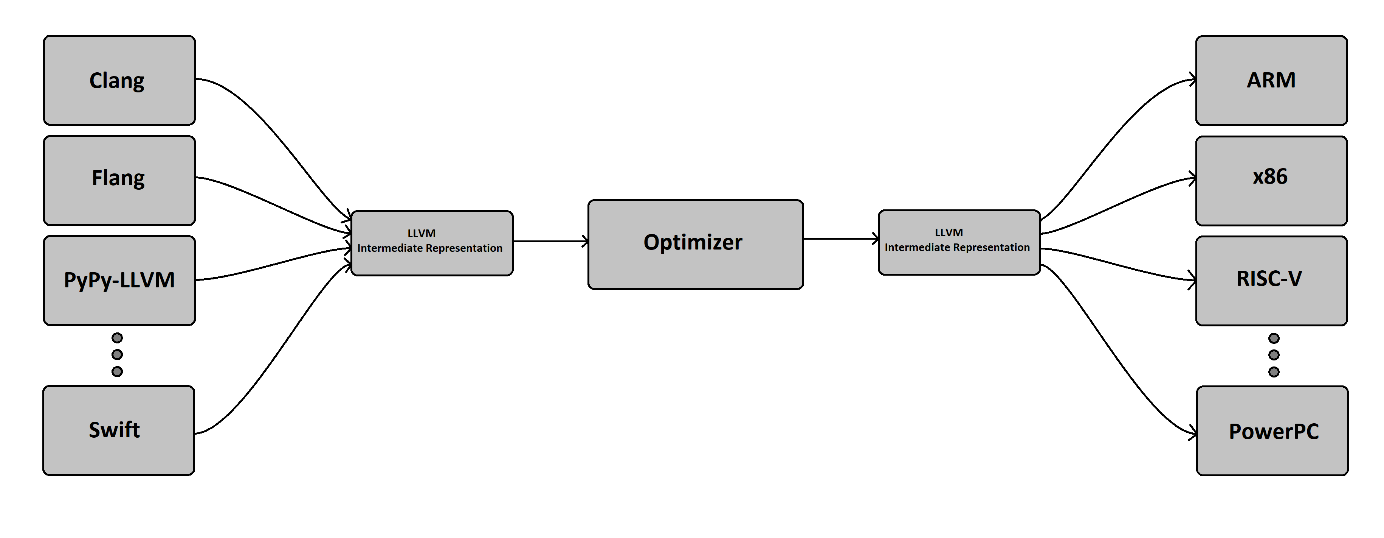
\includegraphics[width=0.8\linewidth]{llvm_diagram.png}
	   \caption{LLVM Frontend ve Backend}
	\end{figure}
\end{frame}

\subsection{LLVM Compiler Backend}
\begin{frame}{Backend}
    \begin{itemize}
        \item Instruction Selection
        \item Scheduling and Formation
        \item SSA based Machine Code Optimizations
        \item Register Allocation
        \item Prolog/Epilog Code Insertion
        \item Code Emission
        \item Linking
        
    \end{itemize}
\end{frame}

\begin{frame}{Instruction Selection Frameworks}
    \begin{itemize}
        \item FastISel
        \item SelectionDAG
        \item GlobalISel
    \end{itemize}
\end{frame}

\begin{frame}{SelectionDAG}
    \begin{enumerate}
    \item 
    Build initial DAG
    \item
    Optimize SelectionDAG
    \item
    Legalize SelectionDAG Types 
    \item
    Optimize SelectionDAG 
    \item
    Legalize SelectionDAG Ops 
    \item
    Optimize SelectionDAG
    \item
    Select instructions from DAG
    \item
    SelectionDAG Scheduling and Formation
    \end{enumerate}

	\begin{definition}
		A \alert{Directed Acyclic Graph (DAG)} is a directed graph with no cycles.
	\end{definition}
\end{frame}

\section{Path from C to Assembly}
\begin{frame}{Target Lowering Steps}
    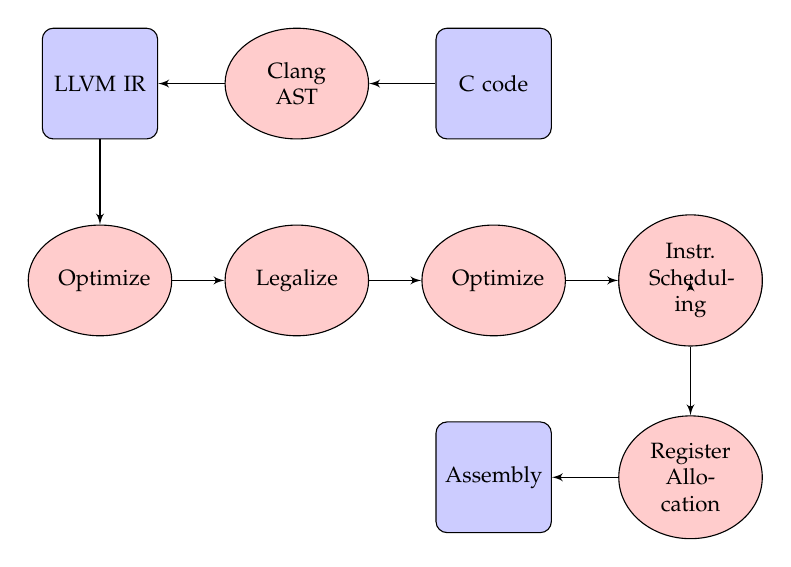
\begin{tikzpicture}[node distance = 2cm, auto]
\centering
\tikzstyle{every node}=[font=\footnotesize]
    % Place nodes
    \node [block] (init) {C code};
    \node [cloud, left of=init,node distance=2.5cm] (ast) {Clang AST};
    \node [block, left of=ast,node distance=2.5cm] (llvmir) {LLVM IR};
    \node [cloud, below of=llvmir,node distance=2.5cm] (opt1) {Optimize};
    \node [cloud, right of=opt1,node distance=2.5cm] (leg) {Legalize};
    \node [cloud, right of=leg,node distance=2.5cm] (opt2) {Optimize};
    \node [cloud, right of=opt2,node distance=2.5cm] (sel) {Instr. Selection};
    \node [cloud, right of=opt2,node distance=2.5cm] (sched) {Instr. Scheduling};
    \node [cloud, below of=sel,node distance=2.5cm] (reg) {Register Allocation};
    \node [block, left of=reg,node distance=2.5cm] (assem) {Assembly};

    % Draw edges
    \path [line] (init) -- (ast);
    \path [line] (ast) -- (llvmir);
    \path [line] (llvmir) -- (opt1);
    \path [line] (opt1) -- (leg);
    \path [line] (leg) -- (opt2);
    \path [line] (opt2) -- (sel);
    \path [line] (sel) -- (sched);
    \path [line] (sched) -- (reg);
    \path [line] (reg) -- (assem);
   
\end{tikzpicture}
\end{frame}

\begin{frame}[fragile]{Example C Code}
\begin{lstlisting}[language=C]
int a,b,c;
void maddFunc() {
	a = 3;
	b = 103;
	c = 127;
	a = a * b + c;
}
\end{lstlisting}
\end{frame}

\begin{frame}[fragile]{LLVM IR}
\lstinputlisting[caption={LLVM IR generated by Clang},label={fig:llvm_ir}, language=llvm, style=nasm]{../thesis/path_instruction/madd.ll}
\end{frame}

\begin{frame}{Initial DAG}
    \begin{figure}
    \centering
    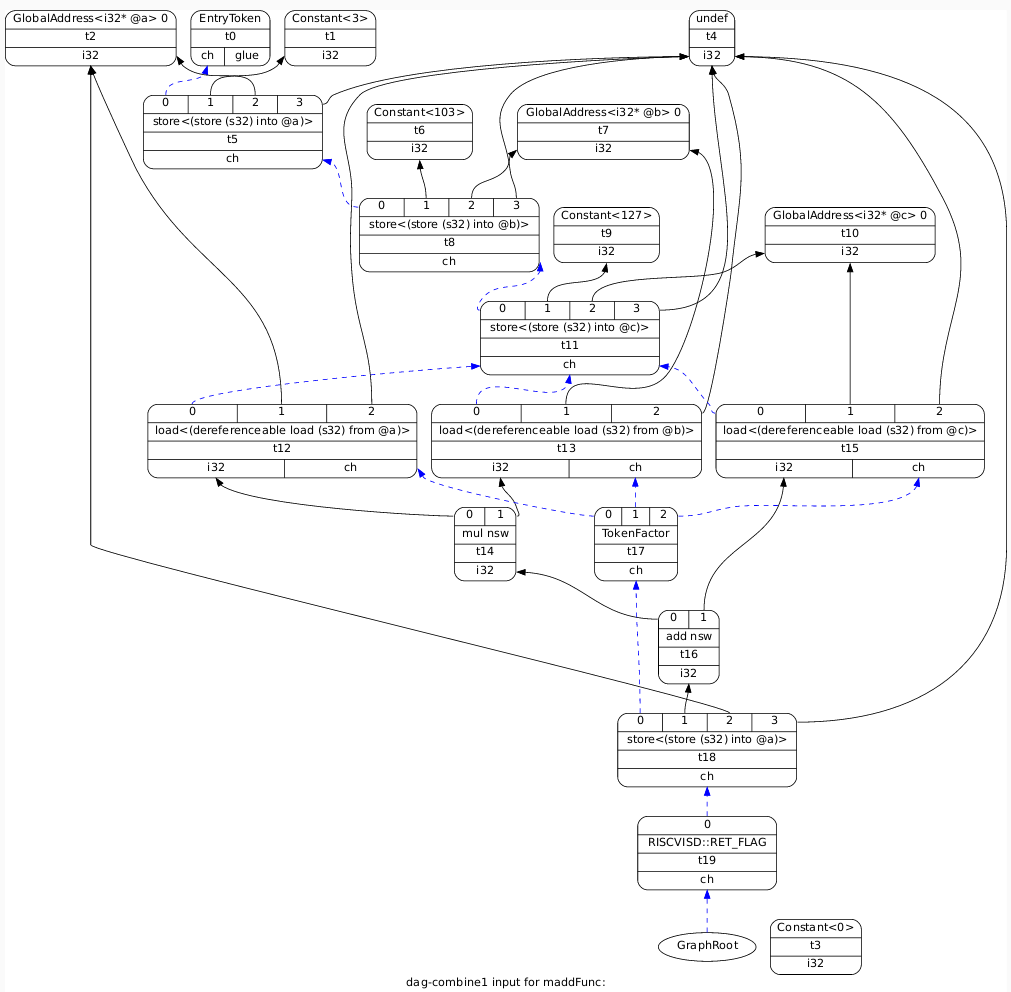
\includegraphics[height=0.75\textheight]{path_instruction/madd_dag_combine1.png}
    \caption{DAG before first optimization pass}
    \label{fig:combine1}
    \end{figure}
\end{frame}

\begin{frame}{DAG After 1st Optimization}
    \begin{figure}
    \centering
    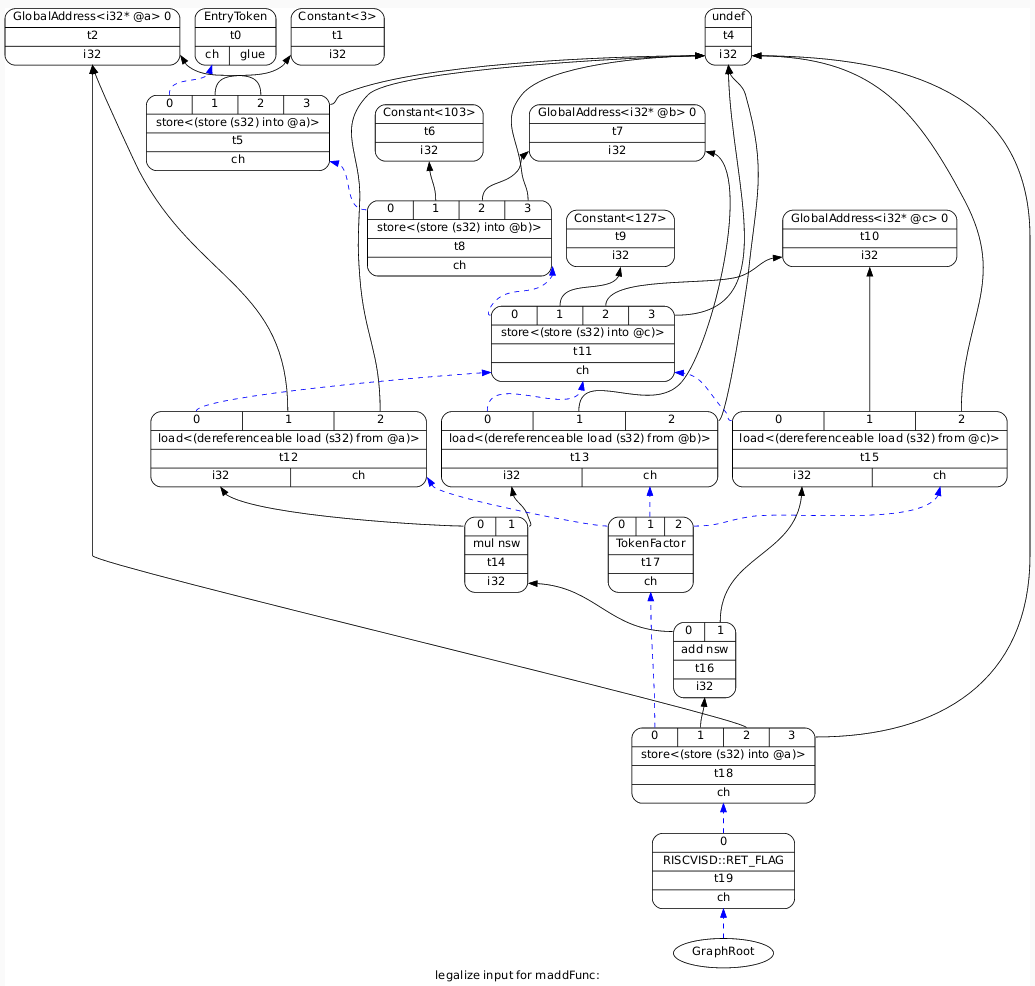
\includegraphics[width=0.77\textheight]{path_instruction/madd_dag_legalize.png}
    \caption{DAG before Legalization}
    \label{fig:legalize}
\end{figure}
\end{frame}

\begin{frame}{DAG After Legalization}
    \begin{figure}
    \centering
    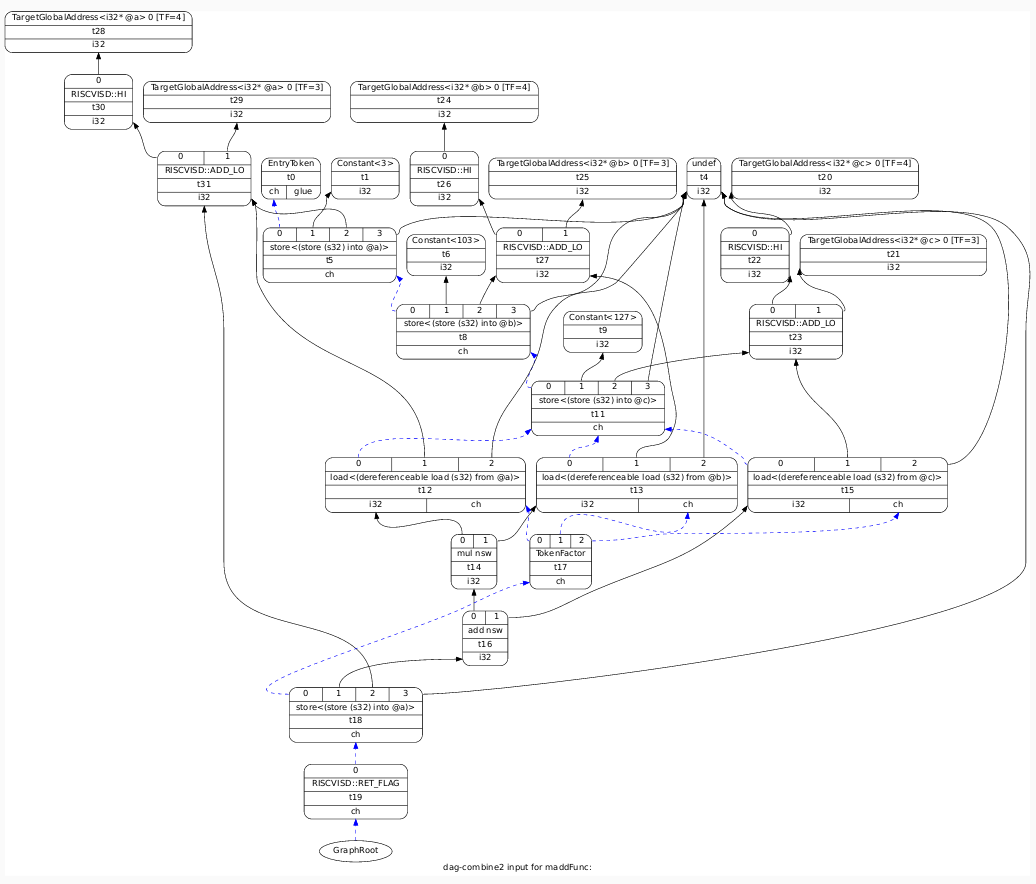
\includegraphics[height=0.75\textheight]{path_instruction/madd_dag_combine2.png}
    \caption{DAG before the second optimization}
    \label{fig:combine2}
\end{figure}
\end{frame}

\begin{frame}{DAG After 2nd Optimization}
    \begin{figure}
    \centering
    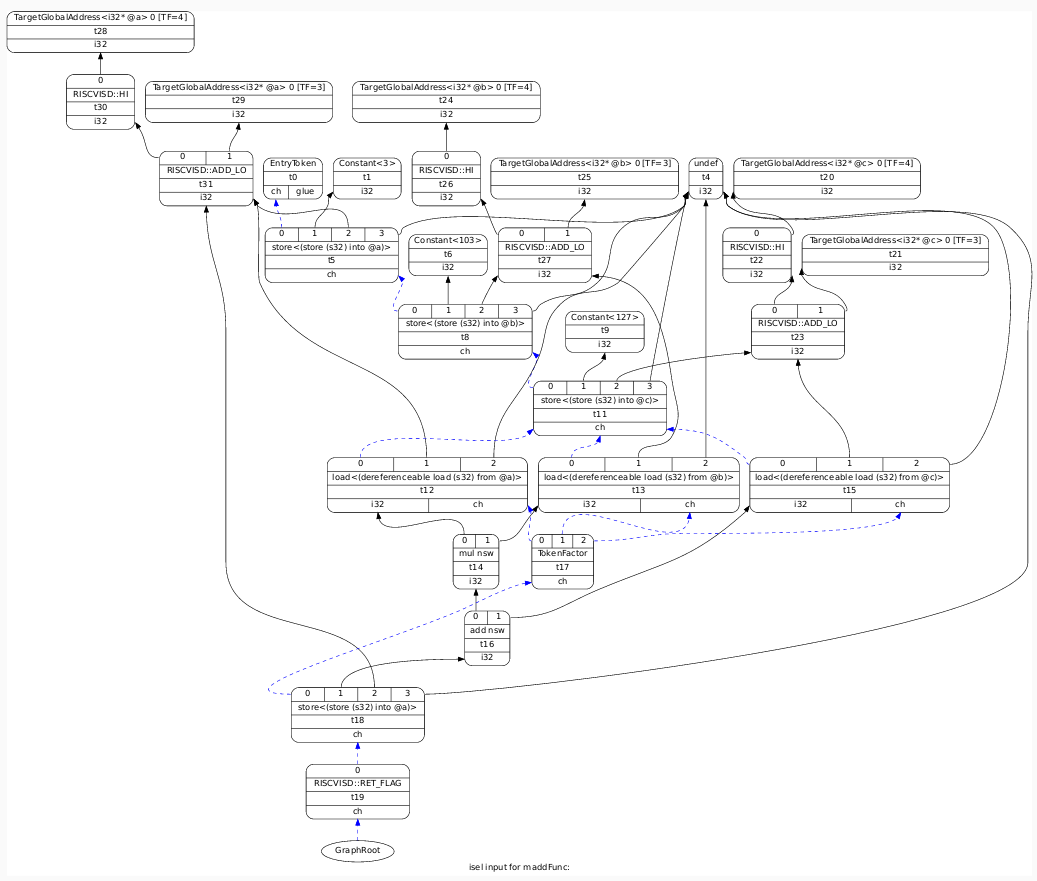
\includegraphics[height=0.75\textheight]{path_instruction/madd_dag_isel.png}
    \caption{DAG before Instruction Selection}
    \label{fig:isel}
\end{figure}
\end{frame}

\begin{frame}{DAG After Instruction Scheduling}
    \begin{figure}
    \centering
    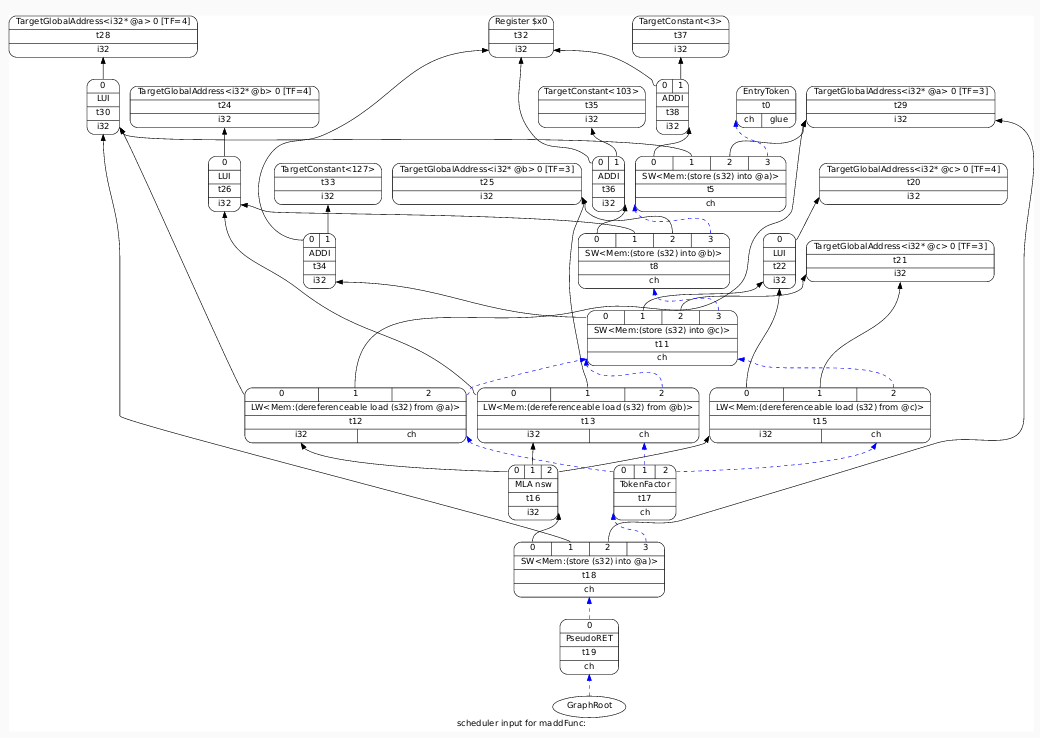
\includegraphics[height=0.75\textheight]{path_instruction/madd_dag_sched.png}
    \caption{DAG before Instruction Scheduling}
    \label{fig:dag_sched}
\end{figure}
\end{frame}

\begin{frame}{Scheduling Dependency Graph}
    \begin{figure}
    \centering
    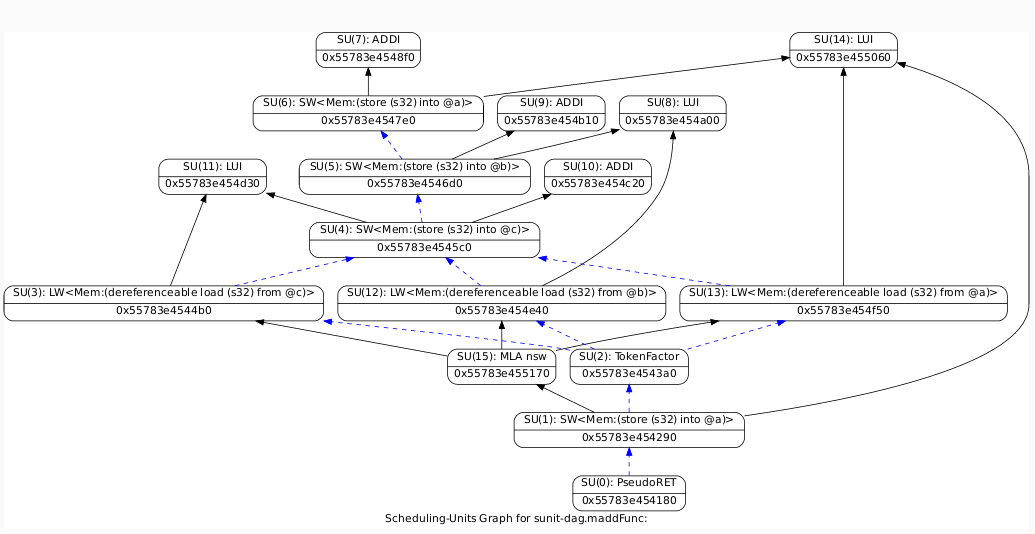
\includegraphics[width=0.85\textwidth]{path_instruction/madd_dag_sunit.png}
    \caption{Scheduling Dependency Graph}
    \label{fig:sunit}
\end{figure}
\end{frame}

\begin{frame}{MachineInstr in SSA Form}
    \begin{figure}
    \centering
    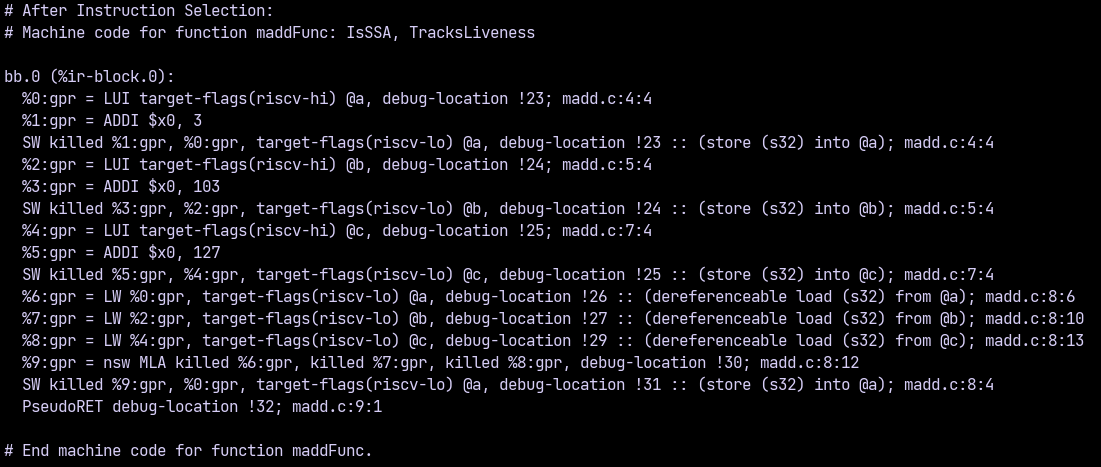
\includegraphics[width=0.85\textwidth]{path_instruction/madd_MachineInstruction.png}
    \caption{MachineInstr before Register Allocation}
    \label{fig:mc_inst}
\end{figure}
\end{frame}

\begin{frame}[fragile]{Final Assembly}
    \begin{lstlisting}[ caption=madd.s Assembly Output]
    ...
	lui	a0, %hi(a)
	li	a1, 3
	sw	a1, %lo(a)(a0)
	lui	a1, %hi(b)
	li	a2, 103
	sw	a2, %lo(b)(a1)
	lui	a2, %hi(c)
	li	a3, 127
	sw	a3, %lo(c)(a2)
	lw	a3, %lo(a)(a0)
	lw	a1, %lo(b)(a1)
	lw	a2, %lo(c)(a2)
	mla	a1, a3, a1 ,a2
	sw	a1, %lo(a)(a0)
	lw	ra, 12(sp)     
	lw	s0, 8(sp)      
    ...
	ret
\end{lstlisting}
\end{frame}

\section{RISC-V Description in SelectionDAG}
\subsection{TableGen Record Declaration}
\begin{frame}{TableGen}
    \begin{itemize}
        \item Domain-specific language used in LLVM backend side to generate CPP header files.
        \item
        Removes redundancy of instruction declaration code
        \item
        Classes are used to convey common information and get inherited to records
        \item
        Declarative instead of Imperative
    \end{itemize}
\end{frame}

\begin{frame}[fragile]{RISC-V TableGen Classes}
Target Independent Instruction Classes
    \begin{itemize}
        \item \textbf{InstructionEncoding}, decoder method, size of instruction
        \item
        \textbf{Instruction}, input and output DAGs
    \end{itemize}
RISC-V Instruction Classes Inherited to declare 'XOR' Instruction
    \begin{itemize}
        \item \textbf{RVInst}, universal bit patterns of RISC-V
        \item
        \textbf{RVInstR}, R type instruction
        \item
        \textbf{ALU\_rr}, features like Commutability declared
    \end{itemize}
\begin{lstlisting}
def XOR  : ALU_rr<0b0000000, 0b100, "xor", /*Commutable*/1>,
           Sched<[WriteIALU, ReadIALU, ReadIALU]>;
\end{lstlisting}
\end{frame}


\subsection{TableGen Pattern Matching}
\begin{frame}[fragile]{TableGen Patterns}
RISC-V TableGen classes can be used to declare any instruction in a more structured way.
\par
The DAG pattern of the instruction can be declared in a Pattern declaration of TableGen. For the NAXOR (NOT AND XOR) instruction, it is: LLVM IR assembly instructions and intrinsic functions are combined in DAG structure.

\begin{lstlisting}
def : Pat< (xor (and (not GPR:$src1), GPR:$src2), GPR:$src3),
(NAXOR GPR:$src1, GPR:$src2, GPR:$src3)>;
\end{lstlisting}
\end{frame}

        
        

\begin{frame}[fragile]{TableGen Patterns}
\begin{lstlisting}
let hasSideEffects = 0, mayLoad = 0, mayStore = 0 in
class ALU_rrr<bits<2> funct2, bits<3> funct3, string opcodestr,
             bit Commutable = 0>
    : RVInstR4<funct2, funct3, OPC_OP, (outs GPR:$rd), (ins GPR:$rs1, GPR:$rs2, GPR:$rs3),
              opcodestr, "$rd, $rs1, $rs2 ,$rs3"> {
  let isCommutable = Commutable;
}
\end{lstlisting}
A custom class of instruction named ALU\_rrr is created. MLA instruction requires three source registers and is defined to be ALU type. 
\end{frame}


        
\begin{frame}[fragile]{TableGen Patterns}
\begin{lstlisting}
def NAXOR     : ALU_rrr<0b11, 0b100, "naxor">,
Sched<[WriteIMul, ReadIMul, ReadIMul]>;
\end{lstlisting}
MLA instruction is defined and ALU\_rrr instruction type is used. funct2,funct3, opcode string and schedules are sufficient to have the full definition of the instruction thanks to the custom ALU\_rrr class.
\end{frame}



\begin{frame}[fragile]{TableGen Patterns}
\begin{figure}
    \centering
    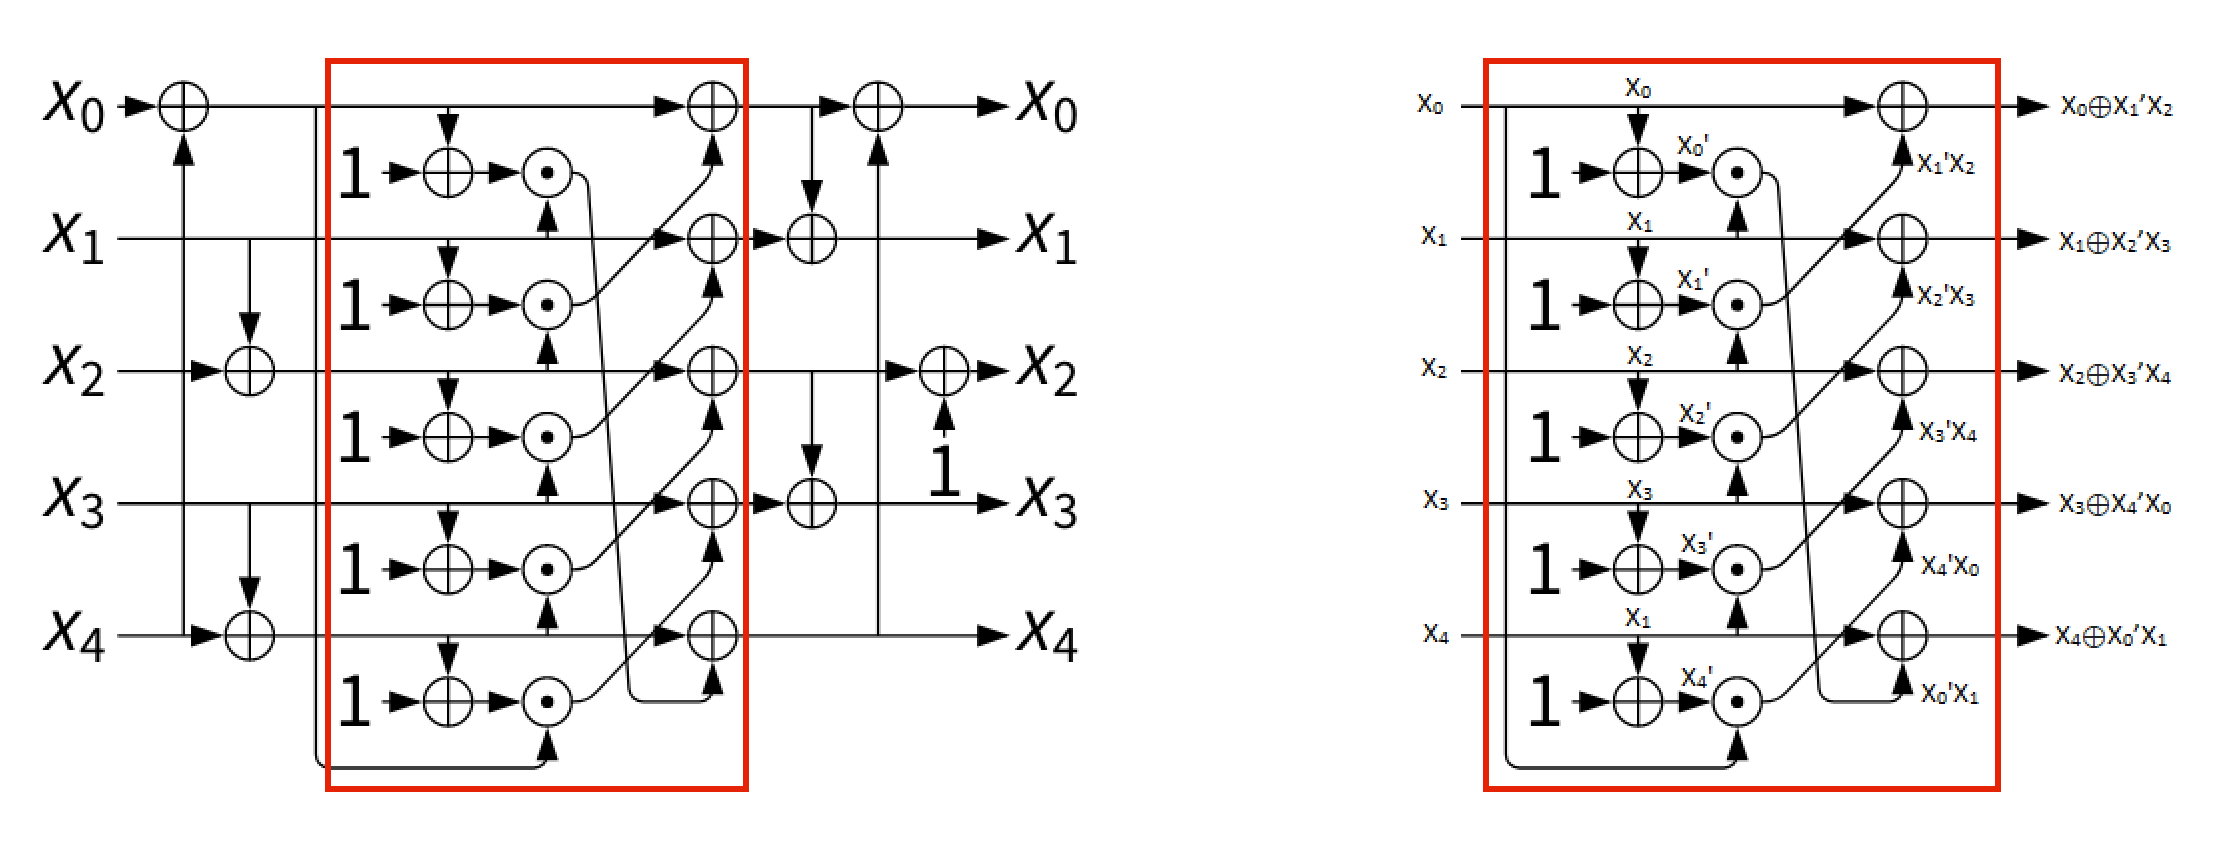
\includegraphics[scale=0.15]{sbox_naxor_pattern.png}
    \caption{NAXOR patterns in s-box algorithm}
    \label{fig:sbox_naxor_pattern}
\end{figure}
This pattern is repeated 5 times as emphasized in Figure \ref{fig:sbox_naxor_pattern}. NAXOR instruction reduces 15 instructions into 5 instructions.
\end{frame}



\begin{frame}[fragile]{TableGen Patterns}
\begin{figure}
    \centering
    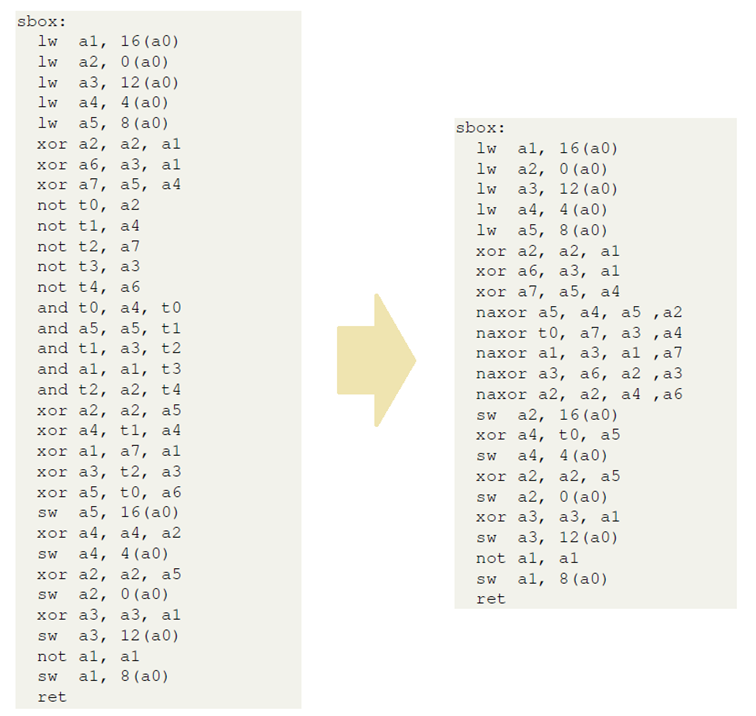
\includegraphics[scale=0.27]{naxor_instruction.png}
    \caption{NAXOR instruction's effect on S-BOX assembly code}
    \label{fig:sbox_instruction}
\end{figure}
The S-box algorithm includes a certain pattern that is used repeatedly.
NOT-AND-XOR pattern is used five times in an s-box cycle. This pattern is lowered
into one instruction using TableGen. After matching this pattern 15 rows of the
assembly file are reduced to one single instruction.
\end{frame}


\section{Pattern Matching with C++}

\subsection{Pattern Matching with C++ in SelectionDAG}
\begin{frame}[fragile]{Limitations of TableGen}
\begin{itemize}
    \item TableGen patterns can only match tree structured patterns.
    \item Cannot match pattern with input relations. All inputs should be independent of each other.
    \item Limited by the language compared to C++.
\end{itemize}

\lstinputlisting[caption={Minimal IR Example of xor(load(x), load(x + 16))},linerange={1-5} ,label={lst:sbox-xor},language=llvm,style=nasm]{../s-box/keccakO3.ll}
\end{frame}

\begin{frame}{Pattern Matching with C++ in SelectionDAG}
\begin{enumerate}
    \item Create a record declaration in TableGen to provide the Assembler support, ignoring the Pattern declaration.
    \item Observe the DAG in the debug output or dot file and locate the root of it. 
    \item Add a function in RISCVISelDAGToDAG.cpp file in the root instruction case. 
    \item Implement pattern matching and replacement with SelectionDAG node.
\end{enumerate}
\end{frame}

\begin{frame}{Example with C++}{LXR Instruction}
\begin{itemize}
    \item Our example instruction LXR, loads two elements from an array and XOR's them.
    \item lxr rd, rs1, rs2 = xor(load(x), load(x + 16))

    \item Because the instruction loads from an array, the address values are relative to each other. 
    \item So TableGen cannot be used for pattern matching.
    \item But TableGen can always be used for instruction encoding thus Assembler support.
\end{itemize}
\end{frame}

\begin{frame}[fragile]{Instruction Encoding of LXR in TableGen}{1.Create a Record}
The input and outputs are registers so TableGen class can used for R-type instructions.

We can override funct7 and funct3 for our custom instruction encoding.
\begin{lstlisting}
let mayLoad = 1 in{
def LXR : ALU_rr<0b0011011, 0b101, "lxr">,
Sched<[WriteIALU, ReadIALU, ReadIALU]>;
}
\end{lstlisting}
llvm-mc assembler can be used for emitting binary from Assembly string.
\end{frame}

\begin{frame}[fragile]{DAG of LXR Pattern}{2.Observe the DAG}
The LXR targeting pattern is produced and dumped in SelectionDAG.
\lstinputlisting[caption={The corresponding Optimized and Legalized DAG}, linerange={3-3,4-4,8-9,13-13,16-16} ,label={lst:sbox-xor-dag},language=llvm,style=nasm]{../s-box/opt-lowered-dag.td}
Instruction Selection works on optimized, legalized DAG in SelectionDAG.
\end{frame}

\begin{frame}[fragile]{Modify RISCVISelDAGToDAG.cpp}{3.Add function call}
    RISCVISelDAGToDAG.cpp contains DAG to DAG transformations in C++.
\lstinputlisting[caption={Introduction of New Function for Pattern Matching in C++},label={lst:sbox-iseldagtodag},language=C++]{../s-box/custom_c++/iseldagtodagPlace.cpp}
\end{frame}


\begin{frame}[fragile]{Pattern Matching Function in C++}{4.Pattern Match Logic}
\lstinputlisting[caption={C++ logic, Part 1}, label={lst:sbox-cpp}, linerange={1-17} ,language=C++]{../s-box/custom_c++/xor_loads.cpp}
\end{frame}

\begin{frame}[fragile]{Pattern Matching Function in C++}{4.Pattern Match Logic}
\lstinputlisting[caption={C++ logic, Part 2}, label={lst:sbox-cpp2}, linerange={19-33} ,language=C++]{../s-box/custom_c++/xor_loads.cpp}
\end{frame}

\begin{frame}{Pattern Checks in the Function}
Check if..
\begin{enumerate}
    \item .. the operands are both Load instructions.
    \item .. the Second Load instruction has an Add instruction in its second operand
    \item .. the base offset of the first load and the first addendum of the second load are the same, as they should point to the beginning of the struct.
    \item .. the second addendum is a constant.
    \item .. the unsigned value of constant second addendum is equal to 16.
\end{enumerate}
\end{frame}

\subsection{Pattern Matching with C++ in Different Levels}


\begin{frame}{Pattern Matching in Different Levels}
It is possible to perform pattern matching in a different level than the backend. 

LLVM IR level and MCInst are the two alternatives for pattern matching.
\begin{center}
    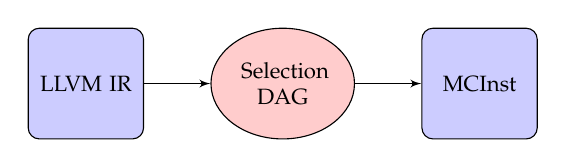
\begin{tikzpicture}[node distance = 2cm, auto]
\tikzstyle{every node}=[font=\footnotesize]
    % Place nodes
    \node [block] (init) {LLVM IR};
    \node [cloud, right of=init,node distance=2.5cm] (ast) {Selection DAG};
    \node [block, right of=ast,node distance=2.5cm] (llvmir) {MCInst};
    % Draw edges
    \path [line] (init) -- (ast);
    \path [line] (ast) -- (llvmir);

   
\end{tikzpicture}
\end{center}
\end{frame}

\begin{frame}{Pattern Matching with LLVM IR}
Rotation operation "ROTR" is matched in LLVM IR in IR level.
    \begin{itemize}
        \item Pattern matching in LLVM IR requires the definition of an intrinsic function.
        \item The intrinsic function is matched in optimization passes according to the pattern.
        \item The matched intrinsics are transferred to the backend and new instruction is emitted.
    \end{itemize}
    Pattern matching in LLVM IR can be more flexible but is more complex to implement.
\end{frame}

\begin{frame}{Pattern Matching with MCInst}
MCInst which is a lower level than SelectionDAG can be used when further detail about instructions are required.

"SH1ADD" is implemented in LLVM by matching materialized immediates. Constants can have different representations and if a specific constant is required, MCInst provides more control to match that. 
\end{frame}




\section{Compiler's Effect on the Code}

\begin{frame}[fragile]{Example C++ Code}
\begin{block}{}
    Quicksort implementation with Lomuto's partition scheme.
\end{block}
\begin{lstlisting}[language=C++]
void quicksort( int low, int high){

    int i;
    if(low < high ){
        i = partition( low, high);
            quicksort( low, i - 1);
            quicksort( i + 1, high);
    }
}
\end{lstlisting}   
\end{frame}
\begin{frame}[fragile]{Example C++ Code}
\begin{lstlisting}[language=C++]
    int partition (int low, int high){
    int i = low;
    int j = low;
    float Pivot = sort.getValue(high); 
    while (sort.getValue(i) <= Pivot && sort.getValue(j) <= Pivot && j < high -1){
        j++;
        i++;
    }
    while ( j < high){
        j++;
        if(sort.getValue(j) < Pivot)
            sort.swap(i,j);
        while(sort.getValue(i) <= Pivot && i < j)
            i++;
    }
    if(j == high)
        sort.swap(i, high);
    return i;
}
\end{lstlisting}
\end{frame}


\begin{frame}{Compiler Optimisations}
    
\begin{figure}
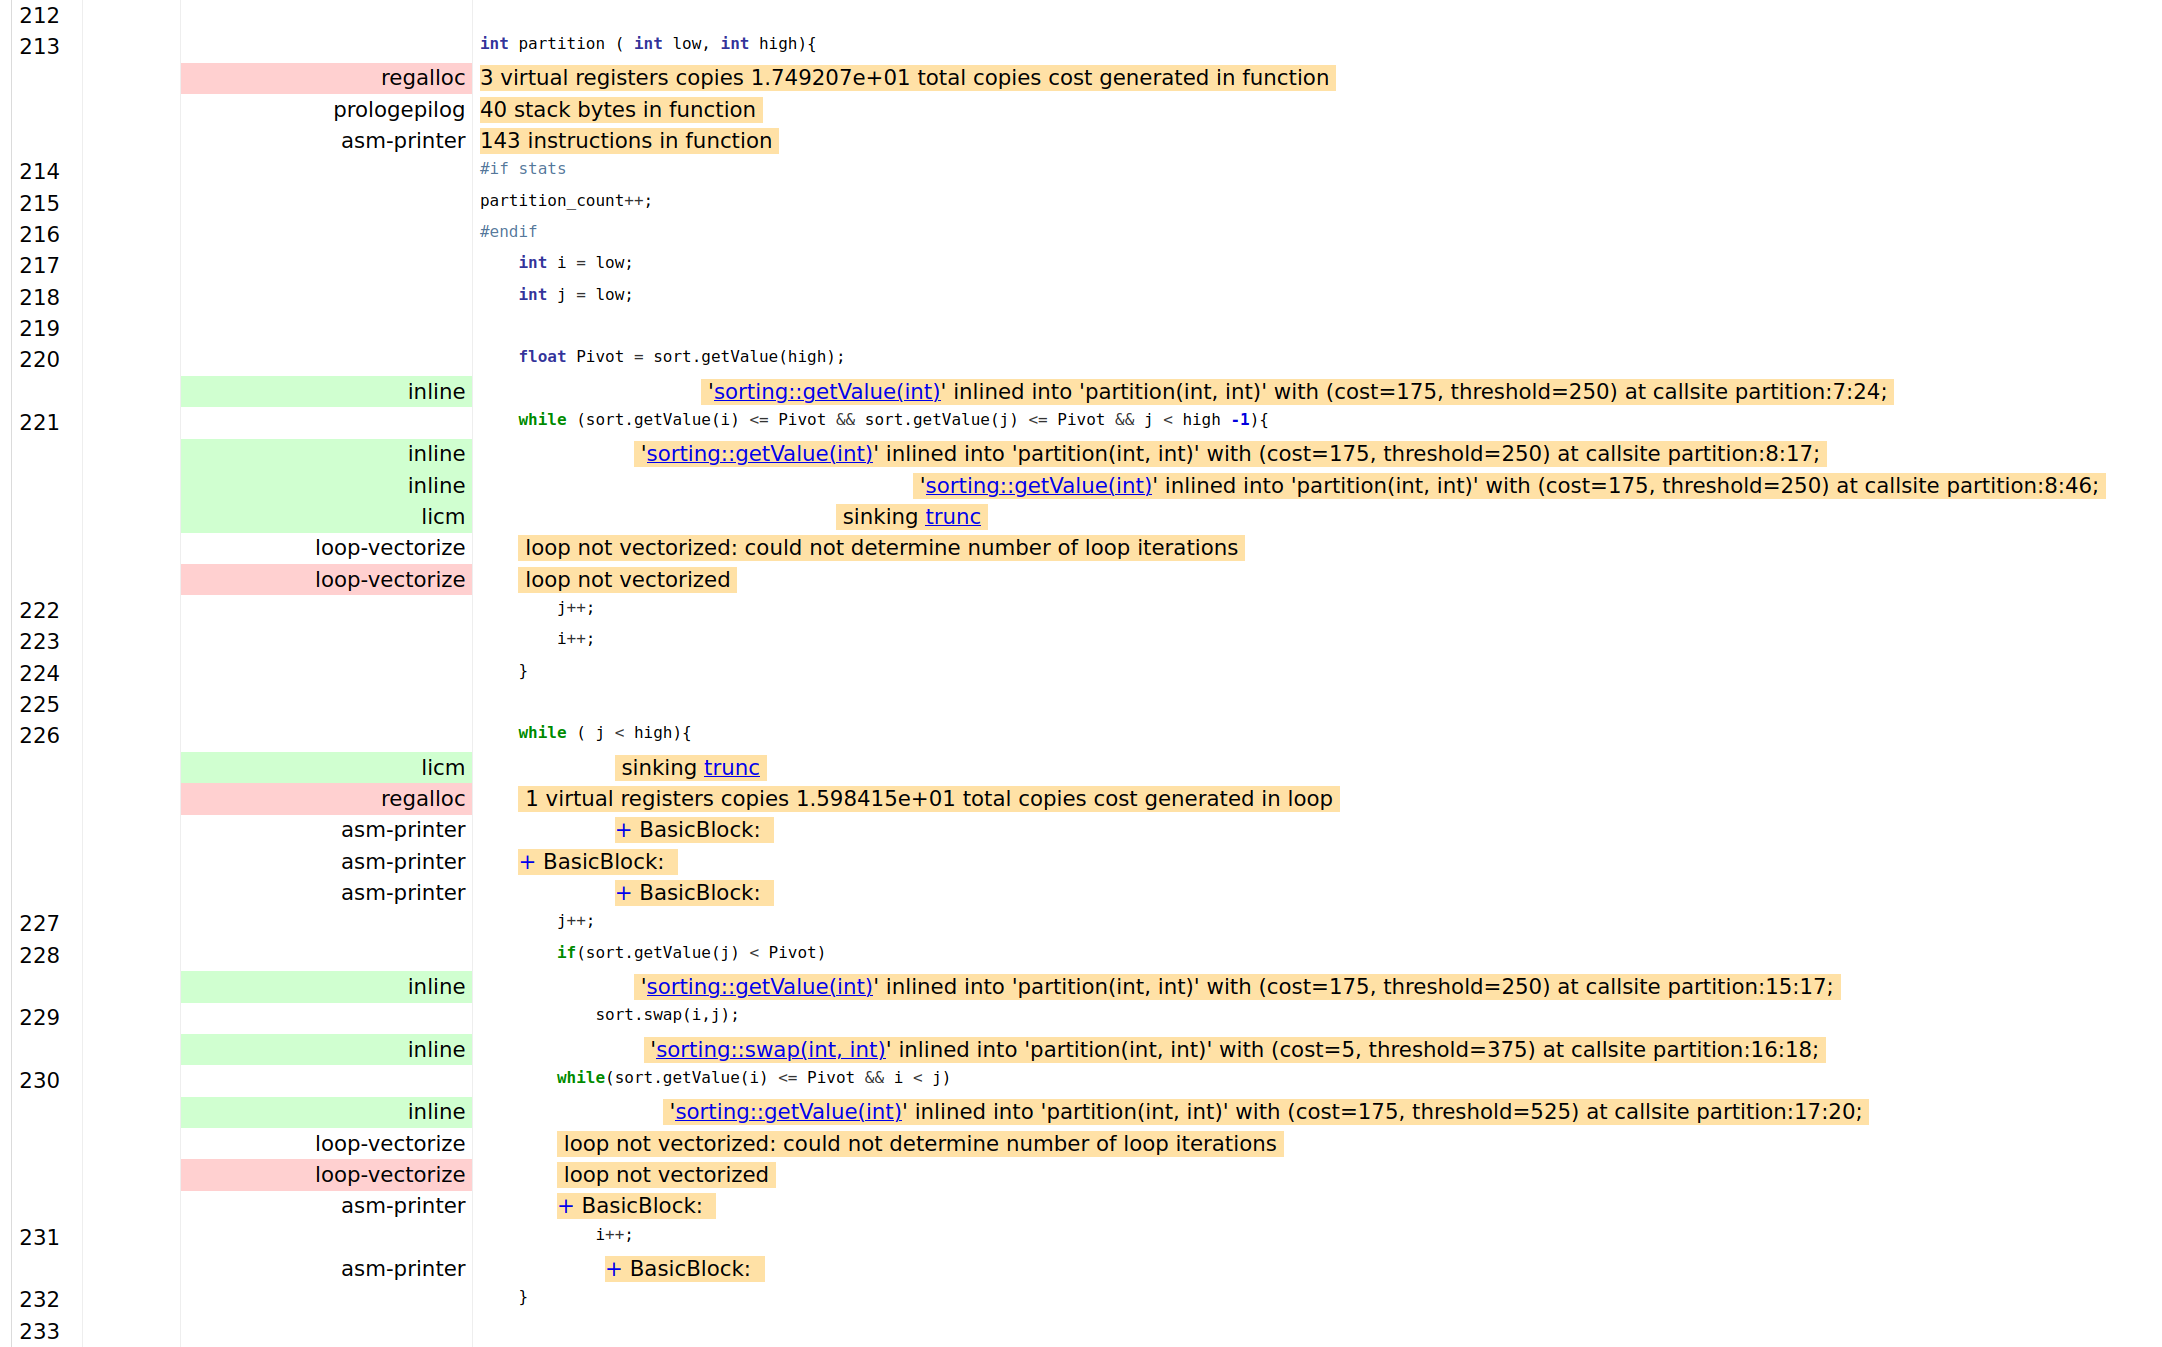
\includegraphics[width=0.8\textwidth]{partition_optviewer.png}
\caption{Optimisations of Clang provided by Opt-Viewer}
\label{part_opt}
\end{figure}
\end{frame}

\begin{frame}{Compiler Optimisations}
    
\begin{figure}
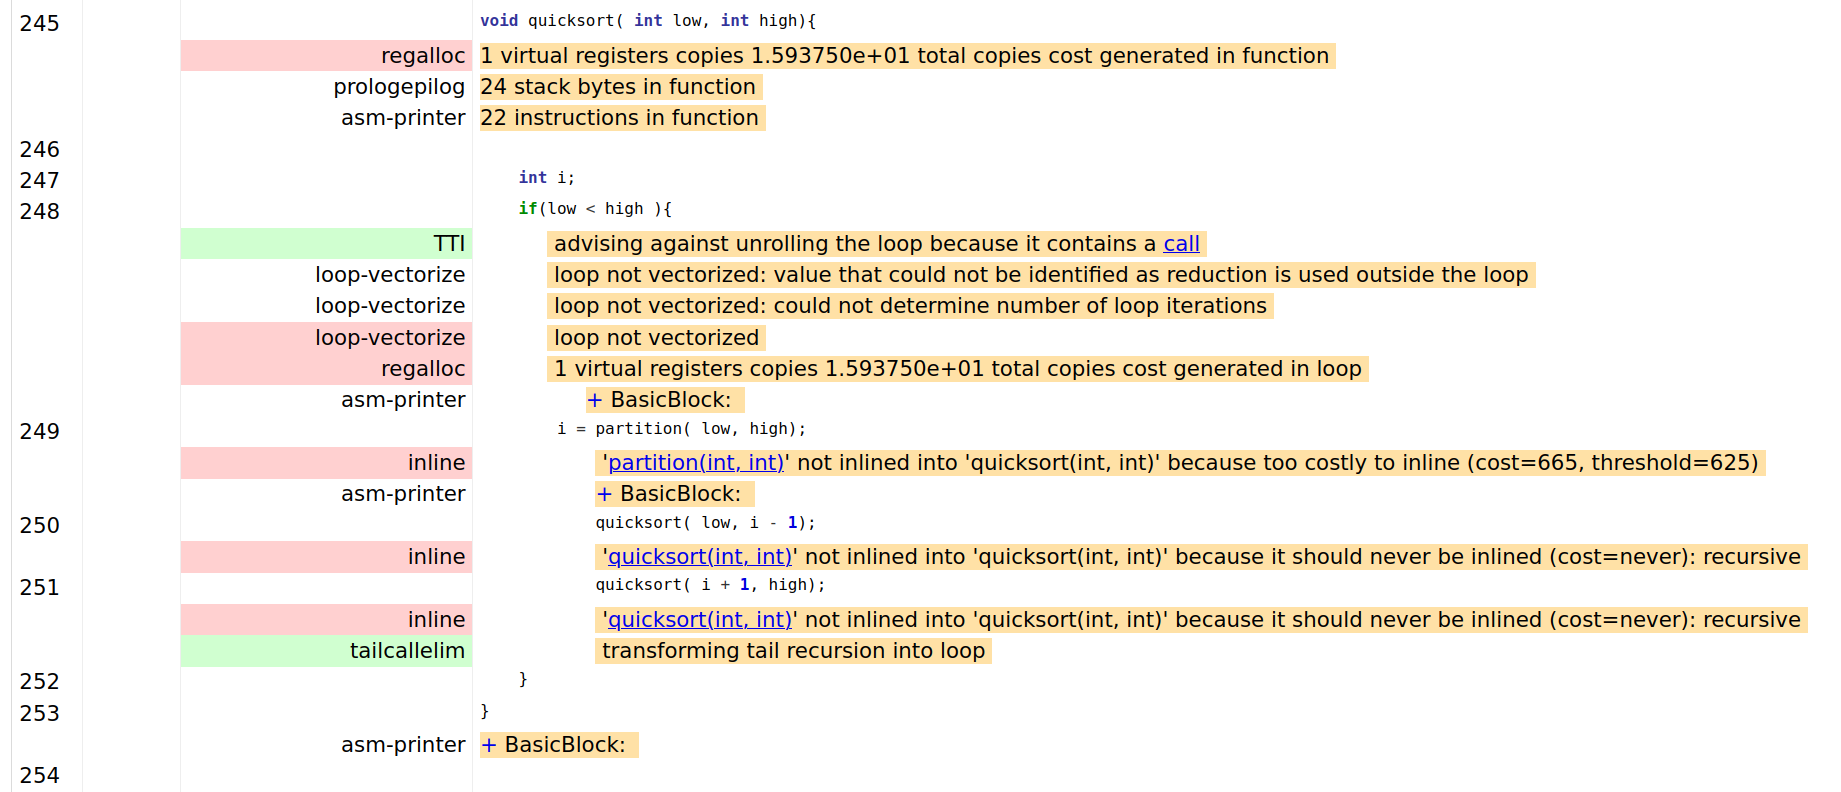
\includegraphics[width=0.8\textwidth]{quicksort_optviewer.png}
\caption{Optimisations of Clang provided by Opt-Viewer}
\label{qs_opt}
\end{figure}
\end{frame}


\end{document} 
